% !TEX program = lualatex
% Web build: latexmlc math152-s8.2-surface-area.tex --dest=surface-area.html --preload=umbc-web.ltxml --css=umbc-latexml.css


\DocumentMetadata{
  lang=en,
  tagging=on,
  pdfstandard=ua-2,
  tagging-setup={math/setup={mathml-AF,mathml-SE}} %methods to store MathML in PDF. AF (associated files) has wider support. SE (structure elements) is newer.
}  % This must come BEFORE \documentclass

\documentclass[10pt,fleqn,leqno]{article}
% 1. Add fleqn here to left-align all math
% 2. Adjust the indent from the left margin (0pt means completely flush)
\setlength{\mathindent}{0pt}

\usepackage[margin=0.85in]{geometry}
\linespread{1.5}
\setlength\parindent{0pt} % no indent
\usepackage{titling}
\setlength{\droptitle}{-2cm} % Pulls the main title up the page

\usepackage{amsmath,amssymb,amsthm}
% LuaLaTeX-only packages (LaTeXML skips these)
\usepackage{tagpdf}
\usepackage{unicode-math}
\tagpdfsetup{math/alt/use}


\usepackage{xcolor}
\definecolor{darkred}{RGB}{139,0,0}
\definecolor{darkblue}{RGB}{0,0,139}

% Define UMBC blue color
\definecolor{umbcblue}{RGB}{0,45,114}

% \usepackage{tcolorbox}
% \usepackage{tabularray}


\usepackage{graphicx}
\graphicspath{ {./images/} }
\usepackage{float}
\usepackage{multicol}
\usepackage[hidelinks]{hyperref}

% \usepackage{tikz}
% \usepackage{pgfplots}
% \pgfplotsset{compat=1.15}

% REDEFINE LIM HERE
\let\oldlim\lim
\renewcommand{\lim}{\displaystyle\oldlim}


\newcommand{\lint}{\displaystyle\int}

\theoremstyle{definition}
\newtheorem{problem}[equation]{Problem}


\usepackage{titling}
\setlength{\droptitle}{-2cm}  % Move title up
\title{\textbf{8.2 Area of a Surface of Revolution}}
\author{}
\date{}

\newcommand{\ddx}{\dfrac{d}{dx}}
\newcommand{\dyx}{\dfrac{dy}{dx}}


%\everymath{\displaystyle}

%Chinese

\usepackage{fontspec}
\newfontfamily\zhfont{PingFang SC}

\begin{document}

\maketitle
\vspace{-5em}

\section*{Surface Area}

Rotating a curve about a line, we obtain a surface of revolution. To find the area of this surface, we slice it into frustum bands, each has the area \( 2\pi \frac{r_1+r_2}{2} L \), where \( r_1, r_2 \) are the lower and upper radii and \( L \) is the slant height.

\begin{center}
	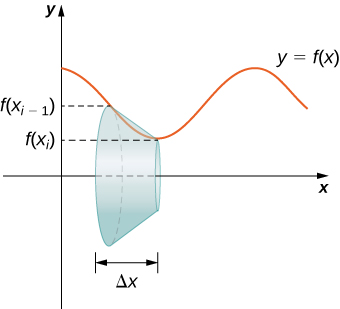
\includegraphics[width=3in,alt={Graph of a curve y = f(x) above the x-axis. Between two nearby points on the x-axis, a distance Delta x apart, the curve is replaced by a straight segment joining the heights f(x sub i minus 1) and f(x sub i). Rotating that segment about the x-axis sweeps out a shaded frustum band, a slice of a cone with circular ends of radius f(x sub i minus 1) and f(x sub i).}]{8-2-frustum}
\end{center}

Compute the area of one band:
\[
	2\pi \underbrace{f(x_i^{**})}_{\text{by IVT}} \, \underbrace{\sqrt{1+\left[ f'(x_i^{*}) \right]^2}\, \Delta x}_{L}
\]

Add up the bands and take the limit to find the surface area:

\textbf{Rotate around the \( x \)-axis.}
\[
	S = \lim_{n\to\infty} \sum_{i=1}^{n} 2\pi f(x_i^{**}) \sqrt{1+\left[ f'(x_i^{*}) \right]^2}\, \Delta x
	= \int_a^b 2\pi f(x) \sqrt{1+\left[ f'(x) \right]^2}\, dx
\]

\textbf{Rotate around the \( y \)-axis.}
\[
	S = \int_c^d 2\pi g(y) \sqrt{1+\left[ g'(y) \right]^2}\, dy
\]

\textbf{In general:}
\[
	S = \int 2\pi r \, ds
\]

\begin{problem}
Let \( f(x)=\sqrt{x} \) on \( [1,4] \). Find the surface area of the surface generated by revolving the graph of \( f(x) \) about the \( x \)-axis.
\end{problem}

\textbf{Solution.}
\[
	f'(x) = \frac{1}{2\sqrt{x}}
\]
\begin{align*}
	S &= \int_1^4 2\pi \sqrt{x}\, \sqrt{1+\frac{1}{4x}}\, dx \\
	  &= \int_1^4 2\pi \sqrt{x+\frac{1}{4}}\, dx \\
	  &= 2\pi \cdot \frac{2}{3} \left( x+\frac{1}{4} \right)^{\frac{3}{2}} \Bigg|_1^4 \\
	  &= \frac{\pi}{6} \left( 17\sqrt{17} - 5\sqrt{5} \right)
\end{align*}

\begin{problem}
Consider \( y=\sqrt[3]{3x} \) for \( 0\le y\le 2 \). Find the surface area of the surface generated by revolving the graph of \( f(x) \) about the \( y \)-axis.
\end{problem}

\textbf{Solution.}
\[
	y^3 = 3x, \qquad x = \frac{y^3}{3}, \qquad \frac{dx}{dy} = y^2
\]
\begin{align*}
	S &= \int_0^2 2\pi\, \frac{y^3}{3} \sqrt{1+y^4}\, dy \\
	  &= \int_0^2 \frac{\pi}{6}\, 4y^3 \sqrt{1+y^4}\, dy \\
	  &= \frac{\pi}{6} \cdot \frac{2}{3} \left( 1+y^4 \right)^{\frac{3}{2}} \Bigg|_0^2 \\
	  &= \frac{\pi}{9} \left( 17^{\frac{3}{2}} - 1 \right)
\end{align*}

\begin{problem}
The curve \( y=\sqrt{4-x^2} \), \( -1\le x\le 1 \), is an arc of the circle \( x^2+y^2=4 \). Find the area of the surface obtained by rotating this arc about the \( x \)-axis.
\end{problem}

\textbf{Solution.}
\[
	y' = \frac{-2x}{2\sqrt{4-x^2}} = \frac{-x}{\sqrt{4-x^2}}
\]
\begin{align*}
	S &= \int_{-1}^{1} 2\pi \sqrt{4-x^2}\, \sqrt{1+\frac{x^2}{4-x^2}}\, dx \\
	  &= \int_{-1}^{1} 2\pi \sqrt{4-x^2+x^2}\, dx \\
	  &= \int_{-1}^{1} 4\pi \, dx \\
	  &= 8\pi
\end{align*}

\section*{Review}

\textbf{Area between curves:}
\begin{align*}
	&\int_a^b f(x)-g(x)\, dx && \text{top} - \text{bottom} \\
	&\int_c^d f(y)-g(y)\, dy && \text{right} - \text{left}
\end{align*}

\textbf{Volume:}
\begin{align*}
	&\text{Disk/washer:} & &\int_a^b \pi \left( R^2-r^2 \right) dx && \text{rotation around the \( x \)-axis} \\
	&\text{Shell:} & &\int_a^b 2\pi x f(x)\, dx && \text{rotation around the \( y \)-axis}
\end{align*}

\textbf{Average value:}
\[
	f_{\text{avg}} = \frac{1}{b-a} \int_a^b f(x)\, dx
\]

\end{document}
